\chapter{Buffer and Schema}

本章介绍缓冲管理与schema设计。Schema部分的内容是一个独立的部分，并不属于存储引擎，放在此处是为了章节的平衡。

\section{缓冲管理}

\section{原生类型}

\section{Schema}

在DMBS中，Schema是一个重要概念，它的核心作用是组织和管理数据库对象（如表、视图、函数、索引等）的逻辑容器。注意，这些对象虽然在同一个Schema中，但是根据对象类型，Schema细分为不同的名字空间。例如，表、视图一般属于一个名字空间，函数、过程属于一个名字空间，索引是一个名字空间，触发器和约束分别对应于不同的名字空间，如\figurename\ref{fig:4-schema}。

\begin{figure}[H]
    \centering
    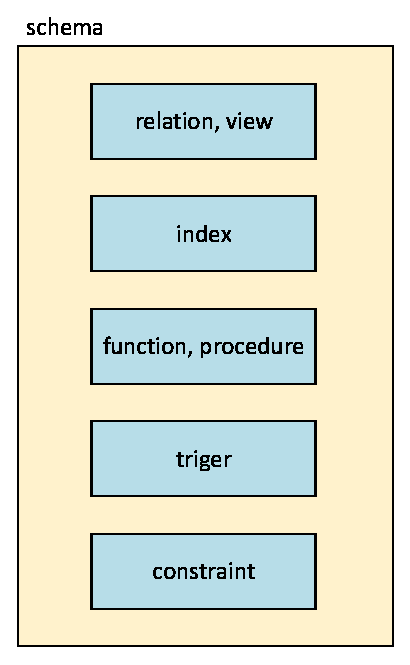
\includegraphics[width=0.4\linewidth]{handout/img/4-schema.eps}
    \caption{schema按照对象类型细分为不同名字空间}\label{fig:4-schema}
\end{figure}

在不同的数据库系统中，schema虽然是一个对象容器，但范畴有些不同。MySQL中最简单，一个库对应于一个schema，库名就是schema名。而在Oracle中，每个用户对应于一个schema，用户名就是schema名。PostgreSQL中，一个库可以创建多个schema，缺省schema为public。SQL server 2005之后，允许一个库有多个schema。从设计初衷来看，多schema主要是为了管理方便，包括权限、逻辑组织等。

MySQL中，一个库对应于一个目录，该库的所有对象（如表、视图、函数、索引等）都存储在该目录下，库的元信息放在系统的数据字典中。PostgreSQL中，一个库的所有文件、索引都放在该库名对应的OID目录下，可以通过库名找到对应的OID，这种设计是为了防止修改库名再去调整目录，PostgreSQL的schema元信息也放在系统数据字典中。

\section{Catalog}





